\documentclass{article}

% packages
\usepackage{amsmath, amsthm, thmtools, amsfonts, amssymb, luacode, catchfile, tikzducks, hyperref, ifthen}
\ifcsname c@kobocompile\endcsname
	\usepackage[a5paper, total={1072pt, 1448pt}, margin=10pt, includeheadfoot]{geometry} % set page margins
\else
	\usepackage[a4paper, margin=50pt, includeheadfoot]{geometry}
\fi
\usepackage[shortlabels]{enumitem}
\usepackage[skip=3pt, indent=0pt]{parskip}

% language
\usepackage[bidi=basic, layout=tabular, provide=*]{babel}
\ifcsname c@english\endcsname
	\babelprovide[main, import]{english}
\else
	\babelprovide[main, import]{hebrew}
	\babelprovide{rl}
\fi
%\babelfont{rm}{Libertinus Serif}
\babelfont{rm}[Renderer=Harfbuzz]{Libertinus Serif}
\babelfont{sf}{Libertinus Sans}
\babelfont{tt}{Libertinus Mono}

% style
\AddToHook{cmd/section/before}{\clearpage}	% Add line break before section
\linespread{1.3}
\setcounter{secnumdepth}{0}		% Remove default number tags from sections, this won't do well with theorems
\AtBeginDocument{\setlength{\belowdisplayskip}{3pt}}
\AtBeginDocument{\setlength{\abovedisplayskip}{3pt}}
\graphicspath{ {../images/} }

% operators
\DeclareMathOperator\cis{cis}
\DeclareMathOperator\Sp{Sp}
\DeclareMathOperator\tr{tr}
\DeclareMathOperator\im{Im}
\DeclareMathOperator\re{Re}
\DeclareMathOperator\diag{diag}
\DeclareMathOperator*\lowlim{\underline{lim}}
\DeclareMathOperator*\uplim{\overline{lim}}
\DeclareMathOperator\rng{rng}
\DeclareMathOperator\Sym{Sym}
\DeclareMathOperator\Arg{Arg}
\DeclareMathOperator\Log{Log}
\DeclareMathOperator\dom{dom}
\DeclareMathOperator\supp{Supp}
\DeclareMathOperator\var{Var}
\DeclareMathOperator\cov{Cov}

% commands
%\renewcommand\qedsymbol{\textbf{מש''ל}}
%\renewcommand\qedsymbol{\fbox{\emoji{lizard}}}
\newcommand{\Aa}[0]{\mathcal{A}}
\newcommand{\Bb}[0]{\mathcal{B}}
\newcommand{\CC}[0]{\mathbb{C}}
\newcommand{\Cc}[0]{\mathcal{C}}
\newcommand{\EE}[0]{\mathbb{E}}
\newcommand{\FF}[0]{\mathbb{F}}
\newcommand{\Ff}[0]{\mathcal{F}}
\newcommand{\Ii}[0]{\mathcal{I}}
\newcommand{\Gg}[0]{\mathcal{G}}
\newcommand{\Ll}[0]{\mathcal{L}}
\newcommand{\Mm}[0]{\mathcal{M}}
\newcommand{\NN}[0]{\mathbb{N}}
\newcommand{\Nn}[0]{\mathcal{N}}
\newcommand{\PP}[0]{\mathbb{P}}
\newcommand{\Pp}[0]{\mathcal{P}}
\newcommand{\QQ}[0]{\mathbb{Q}}
\newcommand{\RR}[0]{\mathbb{R}}
\newcommand{\Rr}[0]{\mathcal{R}}
\newcommand{\Ss}[0]{\mathcal{S}}
\newcommand{\TT}[0]{\mathbb{T}}
\newcommand{\Uu}[0]{\mathcal{U}}
\newcommand{\Vv}[0]{\mathcal{V}}
\newcommand{\Ww}[0]{\mathcal{W}}
\newcommand{\ZZ}[0]{\mathbb{Z}}
\newcommand{\acts}[0]{\circlearrowright}
\newcommand{\explain}[2] {
	\begin{flalign*}
		 && \text{#2} && \text{#1}
	\end{flalign*}
}
\newcommand{\maketitleprint}[0]{ \begin{center}
	%\begin{tikzpicture}[scale=3]
	%	\duck[graduate=gray!20!black, tassel=red!70!black]
	%\end{tikzpicture}	
	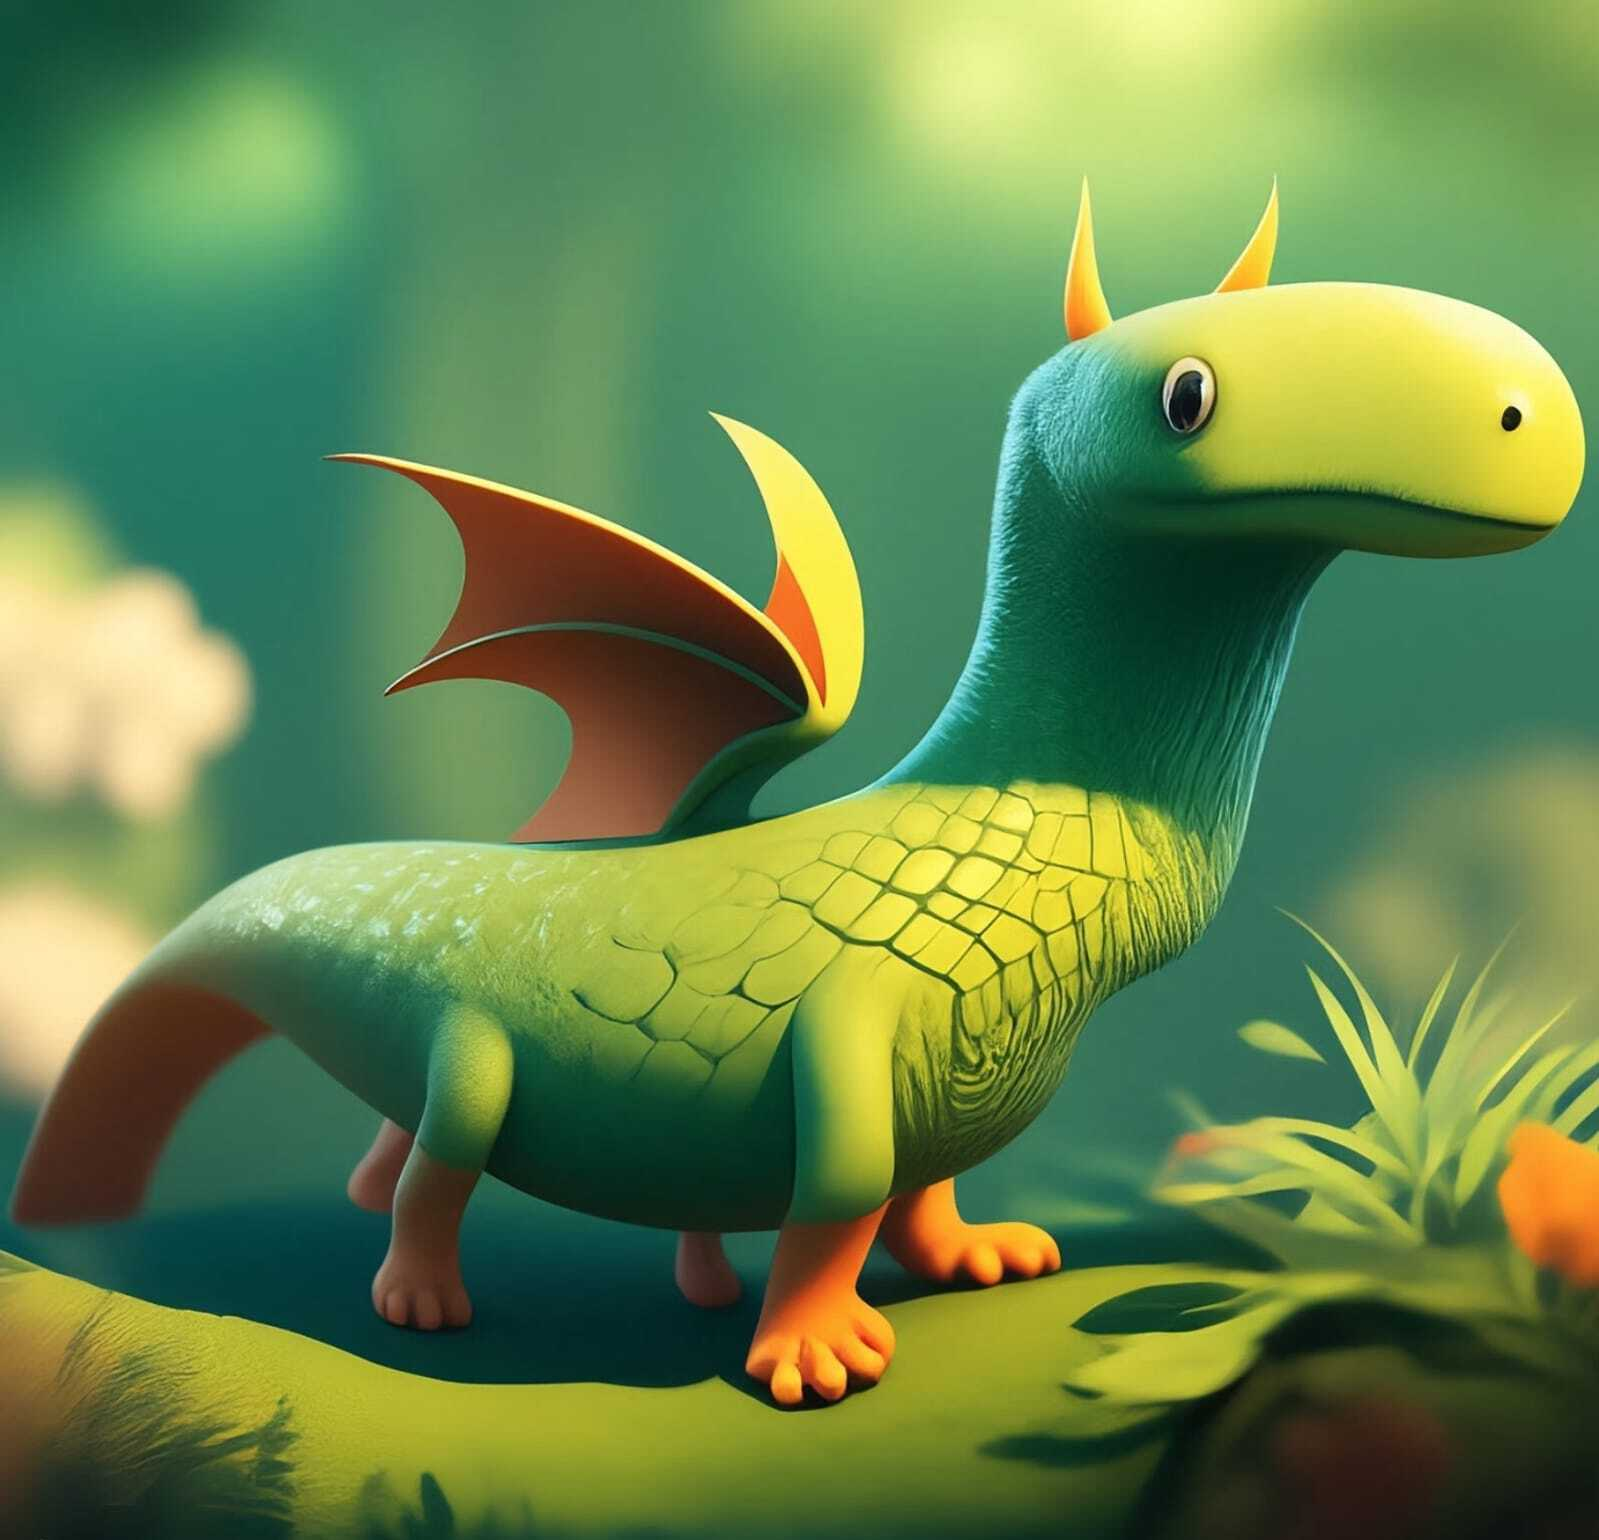
\includegraphics[width=6cm]{cover}
\end{center}
}

% theorem commands
\newtheoremstyle{c_remark}
	{}	% Space above
	{}	% Space below
	{}% Body font
	{}	% Indent amount
	{\bfseries}	% Theorem head font
	{}	% Punctuation after theorem head
	{.5em}	% Space after theorem head
	{\thmname{#1}\thmnumber{ #2}\thmnote{ \normalfont{\text{(#3)}}}}	% head content
\newtheoremstyle{c_definition}
	{3pt}	% Space above
	{3pt}	% Space below
	{}% Body font
	{}	% Indent amount
	{\bfseries}	% Theorem head font
	{}	% Punctuation after theorem head
	{.5em}	% Space after theorem head
	{\thmname{#1}\thmnumber{ #2}\thmnote{ \normalfont{\text{(#3)}}}}	% head content
\newtheoremstyle{c_plain}
	{3pt}	% Space above
	{3pt}	% Space below
	{\itshape}% Body font
	{}	% Indent amount
	{\bfseries}	% Theorem head font
	{}	% Punctuation after theorem head
	{.5em}	% Space after theorem head
	{\thmname{#1}\thmnumber{ #2}\thmnote{ \text{(#3)}}}	% head content

\ifcsname c@english\endcsname
	\theoremstyle{plain}
	\newtheorem{theorem}{Theorem}[section]
	\newtheorem{lemma}[theorem]{Lemma}
	\newtheorem{proposition}[theorem]{Proposition}
	\newtheorem*{proposition*}{Proposition}
	%\newtheorem{corollary}[theorem]{אין חלופה עברית}

	\theoremstyle{definition}
	\newtheorem{definition}[theorem]{Definition}
	\newtheorem*{definition*}{Definition}
	\newtheorem{example}{Example}[section]
	\newtheorem{exercise}{Exercise}[section]

	\theoremstyle{remark}
	\newtheorem*{remark}{Remark}
	\newtheorem*{solution}{Solution}
	\newtheorem{conclusion}[theorem]{Conclusion}
	\newtheorem{notation}[theorem]{Notation}
\else
	\theoremstyle{c_plain}
	\newtheorem{theorem}{משפט}[section]
	\newtheorem{lemma}[theorem]{למה}
	\newtheorem{proposition}[theorem]{טענה}
	\newtheorem*{proposition*}{טענה}
	%\newtheorem{corollary}[theorem]{אין חלופה עברית}

	\theoremstyle{c_definition}
	\newtheorem{definition}[theorem]{הגדרה}
	\newtheorem*{definition*}{הגדרה}
	\newtheorem{example}{דוגמה}[section]
	\newtheorem{exercise}{תרגיל}[section]

	\theoremstyle{c_remark}
	\newtheorem*{remark}{הערה}
	\newtheorem*{solution}{פתרון}
	\newtheorem{conclusion}[theorem]{מסקנה}
	\newtheorem{notation}[theorem]{סימון}
\fi

% Questions related commands
\newcounter{question}
\setcounter{question}{1}
\newcounter{sub_question}
\setcounter{sub_question}{1}

\ifcsname c@english\endcsname
	\newcommand{\question}[1][0]{
		\ifthenelse{#1 = 0}{}{\setcounter{question}{#1}}
		\section{Question \arabic{question}}
		\addtocounter{question}{1}
		\setcounter{sub_question}{1}
	}

	\newcommand{\subquestion}[1][0]{
		\ifthenelse{#1 = 0}{}{\setcounter{sub_question}{#1}}
		\subsection{Part \alph{sub_question}}
		\addtocounter{sub_question}{1}
	}
\else
	\newcommand{\question}[1][0]{
		\ifthenelse{#1 = 0}{}{\setcounter{question}{#1}}
		\section{שאלה \arabic{question}}
		\addtocounter{question}{1}
		\setcounter{sub_question}{1}
	}

	\newcommand{\subquestion}[1][0]{
		\ifthenelse{#1 = 0}{}{\setcounter{sub_question}{#1}}
		\subsection{סעיף \localecounter{letters.gershayim}{sub_question}}
		\addtocounter{sub_question}{1}
	}
\fi

% import lua and start of document
\directlua{common = require ('../common')}

\GetEnv{AUTHOR}

% headers
\author{\AUTHOR}
\date\today

\title{פתרון מטלה 08 --- מבנים אלגבריים (2), 80446}

\begin{document}
\maketitle
\maketitleprint[red]

\question{}
יהי שדה $K$ כך ש־$p\text{-rank}$ של השדה הוא 1, כלומר $[K : K^p] = p^1$.

\subquestion{}
נראה שלכל $n \in \NN$ יש ל־$K$ בדיוק הרחבה אחת $L / K$ שהיא בלתי־ספרבילית לחלוטין מדרגה $p^n$,
וש־$L = K(a^{1 / p^n})$ עבור כל $a \in K \setminus K^p$.
\begin{proof}
	מתכונות $p \text{-rank}$ מתקיים,
	\[
		[K^{1 / p^n} : K]
		=
		[K^{1 / p^n} : K^{1 / p^{n - 1}}]
		\cdots
		[K^{1 / p} : K]
		= {[K : K^p]}^n
		= p^n
	\]
	ולכן נוכל להגדיר $L = K^{1 / p^n}$ ולקבל הרחבה מסדר $p^n$ לש $K$.
	נראה כי היא בלתי בלתי־ספרבילית לחלוטין.
	ממשפט מההרצאה מספיק שנוכיח $L \subseteq K^{1 / p^\infty}$, אבל זה ידוע מהגדרת $K^{1 / p^\infty}$ ולכן $L$ הרחבה בלתי־ספרבילית לחלוטין.

	נניח ש־$L_0 / K$ הרחבה בלתי־ספרבילית לחלוטין מסדר $p^n$, נראה ש־$L_0 = L$. \\
	בלתי־ספרביליות לחלוטין שקולה ל־$L_0 \subseteq K^{1 / p^\infty}$, ו־$[L_0 : K] = p^n$ מאלץ $L_0 \subseteq K^{1 / p^n} \cap K^{1 / p^\infty}$ ולכן $L_0 = L$ בלבד.

	נניח ש־$a \in K \setminus K^p$ איבר שאיננו שורש $p$.
	אז $[K(a^{1 / p^n}) : K] = p^n$ בלבד, ולכן מיחידות $K(a^{1 / p^n}) = L$.
\end{proof}

\subquestion{}
נוכיח שלכל הרחבה סופית $L / K$ יש שדה ביניים $L / L_i / K$ כך ש־$L_i / K$ בלתי־ספרבילית לחלוטין ו־$L / L_i$ ספרבילית.
\begin{proof}
	אנו יודעים כי $[L : K] = p^m$ עבור $m \in \NN$, וכן נבחר $n \le m$ המספר הגדול ביותר כך ש־$L / K^{1 / p^n} / K$, ונסמן $L_i = K^{1 / p^n}$.
	מהסעיף הקודם ברור כי $L_i / K$ בלתי־ספרבילית לחלוטין, ולכן נותר לבדוק את $L / L_i$.
	ישירות מהגדרת $L_i$ אנו יודעים כי אין $\alpha \in L_i$ כך ש־$\alpha$ בלתי־ספרבילי, אחרת מלכתחילה $\alpha \in L_i$, ולכן ${[L : L_i]}_i = 1$ ונובע ש־$L / L_i$ ספרבילי.
\end{proof}

\question{}
נמצא שדה ביניים של ההרחבה $\QQ(\xi_7) / \QQ$ מדרגה $2$ מעל $\QQ$.

\subquestion{}
נמצא תת־חבורה מאינדקס $2$ של $\gal(\QQ(\xi_7) / \QQ) \simeq \ZZ / 6\ZZ$,
ונמצא במפורש אוטומורפיזם $\sigma$ שיוצר אותה.
\begin{solution}
	נגדיר $H = \langle 2 \rangle \le \ZZ / 6\ZZ$, זוהי תת־חבורה מאינדקס $2$.
	היא מתאימה לאוטומורפיזם $\sigma \in \gal(\QQ(\xi_7) / \QQ)$ המוגדר על־ידי,
	\[
		\sigma(\xi_7)
		= \xi_7^2
	\]
\end{solution}

\subquestion{}
נחשב את $z = \sum_{h \in H} h(\xi_7)$ ונראה ש־$h(z) = z$ לכל $h \in H$.
\begin{proof}
	אנו יודעים ש־$\xi_7 \mapsto \xi_7^n$ ל־$n \in {(\ZZ / 7\ZZ)}^\times$ ולכן,
	\[
		z
		= \sum_{h \in H} h(\xi_7)
		= \sum_{n = 1}^6 \xi_7^n
		= -1 + \sum_{n = 0}^6 \xi_7^n
		= -1 + \frac{\xi_7^7 - 1}{\xi_7 - 1}
		= -1
	\]
	בפרט $z \in \QQ$ ו־$h(z) = z$ לכל $h \in \gal(\QQ(\xi_7) / \QQ)$.

	TODO
\end{proof}

\subquestion{}
נסיק ש־$z \in {\QQ(\xi_7)}^H$ וש־$[\QQ(z) : \QQ] \le 2$.
\begin{proof}
	TODO
\end{proof}

\question{}
יהי $K$ שדה, ו־$f \in K[x]$ אי־פריק וספרבילי.
נניח גם כי $L$ שדה פיצול של $f$ מעל $K$.

\subquestion{}
נראה שאם כל שדה ביניים $L / E / K$ הוא נורמלי אז כל שורש של $f$ יוצר את $L$ מעל $K$.
\begin{proof}
	יהי $\alpha$ שורש של $f$, אז $L / K(\alpha) / K$ הרחבה נורמלית, ו־$f_{\alpha, K}$ מתפצל לחלוטין בשדה זה.
	אבל $f = f_{\alpha, K}$ ישירות מהגדרה, כלומר $K(\alpha) = L$ בלבד.
\end{proof}

\subquestion{}
נסיק שאם $\gal(L / K)$ אבלית אז כל שורש של $f$ יוצר את $L$ מעל $K$.
\begin{proof}
	בחבורה אבלית כל תת־חבורה היא תת־חבורה נורמלית של החבורה, לכן אם $N \le \gal(L / K)$ אז $N \trianglelefteq \gal(L / K)$ ו־$L^N / K$ הרחבה נורמלית של $K$.
	מהסעיף הקודם נסיק ישירות שכל שורש של $f$ יוצר את $L$ מעל $K$.
\end{proof}

\question{}
נסמן $f(x) = x^4 - 7x^2 + 7 \in \QQ[x]$, ונניח כי $L / \QQ$ שדה פיצול של $f$.

\subquestion{}
נסמן,
\[
	\beta_1
	= \frac{7 + \sqrt{21}}{2},
	\quad
	\beta_2
	= \frac{7 - \sqrt{21}}{2}
\]
השורשים של $y^2 - 7y + 7 = 0$.

\subquestion{}
נראה ש־$\QQ(\beta_1, \beta_2) = \QQ(\beta_1)$ וש־$[\QQ(\sqrt{\beta_1}, \sqrt{\beta_2}) : \QQ(\beta_1)] = 4$.
\begin{proof}
	מתקיים,
	\[
		\beta_2
		= 7 - \beta_1
	\]
	ו־$7 \in \QQ$ לכן $\beta_2 \in \QQ(\beta_1)$ ובהתאם $\QQ(\beta_1, \beta_2) = \QQ(\beta_1)$ ובפרט $\QQ(\beta_1) = \QQ(\beta_2)$.

	כהיסק ישיר גם,
	\[
		[\QQ(\sqrt{\beta_1}, \sqrt{\beta_2}) : \QQ(\beta_1)]
		= [\QQ(\sqrt{\beta_1}, \sqrt{\beta_2}) : \QQ(\sqrt{\beta_1})]
		\cdot [\QQ(\sqrt{\beta_1}) : \QQ(\beta_1)]
		= 2 \cdot 2
	\]
	כמסקנה ממטלה 5 שאלה 3 סעיף ב'.
\end{proof}

\subquestion{}
נסיק ש־$L = \QQ(\sqrt{\beta_1}, \sqrt{\beta_2})$ מדרגה 8 מעל $\QQ$.
\begin{proof}
	אנו יודעים כי $[\QQ(\beta_1) : \QQ] = 2$ כשורש של פולינום אי־פריק ב־$\QQ$ מסדר 2, ולכן,
	\[
		[L : \QQ]
		= [L : \QQ(\beta_1)] \cdot [\QQ(\beta_1) : \QQ]
		= 4 \cdot 2
	\]
	וקיבלנו כי הדרגה היא $8$.
\end{proof}

\subquestion{}
נמצא את טיפוס האיזומורפיזם של $\gal(L / \QQ)$.
\begin{solution}
	אנו יודעים כי $|\gal(L / \QQ)| = 8$. \\
	אנו גם יודעים כי כל אוטומורפיזם $\sigma \in \gal(L / \QQ)$ נקבע ביחידות על־ידי המיפוי שלו ל־$\beta_1, \sqrt{\beta_1}, \sqrt{\beta_2}$, ושמיפוי זה בלתי תלוי,
	לכן נסיק ש־$\gal(L / \QQ) \simeq \HH$, חבורת הקוונטרניונים.
\end{solution}

\end{document}
